  \documentclass[oneside]{book}
%\documentclass[12pt,]{book}

\usepackage{lmodern}
\usepackage{setspace}
\setstretch{2}
\usepackage{amssymb,amsmath}
\usepackage{ifxetex,ifluatex}
\usepackage{fixltx2e} % provides \textsubscript
\ifnum 0\ifxetex 1\fi\ifluatex 1\fi=0 % if pdftex
  \usepackage[T1]{fontenc}
  \usepackage[utf8]{inputenc}
\else % if luatex or xelatex
  \ifxetex
    \usepackage{xltxtra,xunicode}
  \else
    \usepackage{fontspec}
  \fi
  \defaultfontfeatures{Ligatures=TeX,Scale=MatchLowercase}


\fi
% use upquote if available, for straight quotes in verbatim environments
\IfFileExists{upquote.sty}{\usepackage{upquote}}{}
% use microtype if available
\IfFileExists{microtype.sty}{%
\usepackage{microtype}
\UseMicrotypeSet[protrusion]{basicmath} % disable protrusion for tt fonts
}{}
\usepackage[a4paper, left=1.18in, right=1.18in, top=1.18in, bottom=0.787in]{geometry}
\usepackage[unicode=true]{hyperref}
\hypersetup{
            pdftitle={臺灣大學論文 Bookdown 模板},
            pdfauthor={廖永賦},
            pdfborder={0 0 0},
            breaklinks=true}
\urlstyle{same}  % don't use monospace font for urls
\usepackage{color}
\usepackage{fancyvrb}
\newcommand{\VerbBar}{|}
\newcommand{\VERB}{\Verb[commandchars=\\\{\}]}
\DefineVerbatimEnvironment{Highlighting}{Verbatim}{commandchars=\\\{\}}
% Add ',fontsize=\small' for more characters per line
\usepackage{framed}
\definecolor{shadecolor}{RGB}{248,248,248}
\newenvironment{Shaded}{\begin{snugshade}}{\end{snugshade}}
\newcommand{\KeywordTok}[1]{\textcolor[rgb]{0.13,0.29,0.53}{\textbf{#1}}}
\newcommand{\DataTypeTok}[1]{\textcolor[rgb]{0.13,0.29,0.53}{#1}}
\newcommand{\DecValTok}[1]{\textcolor[rgb]{0.00,0.00,0.81}{#1}}
\newcommand{\BaseNTok}[1]{\textcolor[rgb]{0.00,0.00,0.81}{#1}}
\newcommand{\FloatTok}[1]{\textcolor[rgb]{0.00,0.00,0.81}{#1}}
\newcommand{\ConstantTok}[1]{\textcolor[rgb]{0.00,0.00,0.00}{#1}}
\newcommand{\CharTok}[1]{\textcolor[rgb]{0.31,0.60,0.02}{#1}}
\newcommand{\SpecialCharTok}[1]{\textcolor[rgb]{0.00,0.00,0.00}{#1}}
\newcommand{\StringTok}[1]{\textcolor[rgb]{0.31,0.60,0.02}{#1}}
\newcommand{\VerbatimStringTok}[1]{\textcolor[rgb]{0.31,0.60,0.02}{#1}}
\newcommand{\SpecialStringTok}[1]{\textcolor[rgb]{0.31,0.60,0.02}{#1}}
\newcommand{\ImportTok}[1]{#1}
\newcommand{\CommentTok}[1]{\textcolor[rgb]{0.56,0.35,0.01}{\textit{#1}}}
\newcommand{\DocumentationTok}[1]{\textcolor[rgb]{0.56,0.35,0.01}{\textbf{\textit{#1}}}}
\newcommand{\AnnotationTok}[1]{\textcolor[rgb]{0.56,0.35,0.01}{\textbf{\textit{#1}}}}
\newcommand{\CommentVarTok}[1]{\textcolor[rgb]{0.56,0.35,0.01}{\textbf{\textit{#1}}}}
\newcommand{\OtherTok}[1]{\textcolor[rgb]{0.56,0.35,0.01}{#1}}
\newcommand{\FunctionTok}[1]{\textcolor[rgb]{0.00,0.00,0.00}{#1}}
\newcommand{\VariableTok}[1]{\textcolor[rgb]{0.00,0.00,0.00}{#1}}
\newcommand{\ControlFlowTok}[1]{\textcolor[rgb]{0.13,0.29,0.53}{\textbf{#1}}}
\newcommand{\OperatorTok}[1]{\textcolor[rgb]{0.81,0.36,0.00}{\textbf{#1}}}
\newcommand{\BuiltInTok}[1]{#1}
\newcommand{\ExtensionTok}[1]{#1}
\newcommand{\PreprocessorTok}[1]{\textcolor[rgb]{0.56,0.35,0.01}{\textit{#1}}}
\newcommand{\AttributeTok}[1]{\textcolor[rgb]{0.77,0.63,0.00}{#1}}
\newcommand{\RegionMarkerTok}[1]{#1}
\newcommand{\InformationTok}[1]{\textcolor[rgb]{0.56,0.35,0.01}{\textbf{\textit{#1}}}}
\newcommand{\WarningTok}[1]{\textcolor[rgb]{0.56,0.35,0.01}{\textbf{\textit{#1}}}}
\newcommand{\AlertTok}[1]{\textcolor[rgb]{0.94,0.16,0.16}{#1}}
\newcommand{\ErrorTok}[1]{\textcolor[rgb]{0.64,0.00,0.00}{\textbf{#1}}}
\newcommand{\NormalTok}[1]{#1}
\usepackage{longtable,booktabs}
% Fix footnotes in tables (requires footnote package)
\IfFileExists{footnote.sty}{\usepackage{footnote}\makesavenoteenv{long table}}{}
\let\oldhref=\href
% Make links footnotes instead of hotlinks:
\renewcommand{\href}[2]{#2\footnote{\url{#1}}}
\IfFileExists{parskip.sty}{%
\usepackage{parskip}
}{% else
\setlength{\parindent}{0pt}
\setlength{\parskip}{6pt plus 2pt minus 1pt}
}
\setlength{\emergencystretch}{3em}  % prevent overfull lines
\providecommand{\tightlist}{%
  \setlength{\itemsep}{0pt}\setlength{\parskip}{0pt}}
\setcounter{secnumdepth}{2}

% set default figure placement to htbp
\makeatletter
\def\fps@figure{htbp}
\makeatother

\usepackage{pdfpages}
\usepackage{titlesec}
\usepackage{titletoc}
\usepackage{xCJKnumb}
\usepackage{booktabs}


%中文自動換行
\XeTeXlinebreaklocale "zh"
%文字的彈性間距
\XeTeXlinebreakskip = 0pt plus 1pt


\titleformat{\chapter}{\centering\Huge\bfseries}{第\,\xCJKnumber{\thechapter}\,章}{1em} {}
\titlespacing{\chapter}{0cm}{-1.3cm}{1em} 

\renewcommand{\figurename}{圖}
\renewcommand{\tablename}{表}
\renewcommand{\contentsname}{目錄}
\renewcommand{\listfigurename}{圖目錄}
\renewcommand{\listtablename}{表目錄}
%\renewcommand{\bibname}{參考資料}

\titlecontents{chapter}[0em]
{}{\makebox[4.1em][l]
{第\xCJKnumber{\thecontentslabel}章}}{}
{\titlerule*[0.7pc]{.}\contentspage}

\title{臺灣大學論文 Bookdown 模板}
\author{廖永賦}
\date{October 30, 2018}


\usepackage{fontspec}
%使用xeCJK,其他的還有CJK或是xCJK
\usepackage{xeCJK}
\usepackage{bm}

% Set the default fonts
  \setmainfont{Liberation Serif} % Times New Roman  %Liberation Serif

            \setCJKmainfont[
	    BoldFont={AR PL KaitiM Big5}  % 粗體字
        ]{AR PL KaitiM Big5}
    


% IPA support (Works with linguisticsdown)
  \newfontfamily\ipa{Doulos SIL} % Font for IPA symbols
  \DeclareTextFontCommand{\ipatext}{\ipa}


\usepackage{xcolor}
\usepackage{transparent}
\usepackage[printwatermark]{xwatermark}

  \newwatermark*[allpages,xpos=6.1725cm,ypos=10.5225cm,scale=0.5]{
\includegraphics{watermark.pdf}}


\begin{document}



\includepdf[pages={1}, scale=1]{front_matter/front_matter.pdf}

\clearpage
\pagenumbering{roman}

\phantomsection
\addcontentsline{toc}{chapter}{口試委員會審定書}

\includepdf[pages={1}, scale=1]{certification-scan.pdf}

\phantomsection
\addcontentsline{toc}{chapter}{誌謝}

\includepdf[pages={3}, scale=1]{front_matter/front_matter.pdf}


\phantomsection
\addcontentsline{toc}{chapter}{中文摘要}

\includepdf[pages={4}, scale=1]{front_matter/front_matter.pdf}

\phantomsection
\addcontentsline{toc}{chapter}{英文摘要}

\includepdf[pages={5}, scale=1]{front_matter/front_matter.pdf}

\clearpage
\pagenumbering{arabic}

{
\setcounter{tocdepth}{1}
\tableofcontents
}

\newpage

\listoftables
\newpage
\listoffigures
\newpage

% Set independent linestretch for code chunks
\let\oldShaded=\Shaded
\let\endoldShaded=\endShaded
\renewenvironment{Shaded}{
      \begin{spacing}{1.5}\begin{oldShaded}
    }
  {
  \end{oldShaded}
  \end{spacing}
  }


\chapter{Introduction}\label{intro}

中文文獻 (黃宣範, \protect\hyperlink{ref-huangxuanfan1993}{1993})

english citation (Leung, Maddux, Galinsky, \& Chiu,
\protect\hyperlink{ref-leung2008}{2008}).

\chapter{安裝}\label{install}

\begin{Shaded}
\begin{Highlighting}[]
\NormalTok{devtools}\OperatorTok{::}\KeywordTok{install_github}\NormalTok{(}\StringTok{"liao961120/ntuthesis"}\NormalTok{)}
\end{Highlighting}
\end{Shaded}

\section{LaTeX}\label{latex}

若已有管理、安裝 LaTeX 套件經驗者,可忽略。

若電腦尚未安裝 LaTeX,可安裝 R 的 tinytex 套件:

\begin{Shaded}
\begin{Highlighting}[]
\KeywordTok{install.packages}\NormalTok{(}\StringTok{'tinytex'}\NormalTok{)}
\NormalTok{tinytex}\OperatorTok{::}\KeywordTok{install_tinytex}\NormalTok{()}
\end{Highlighting}
\end{Shaded}

在輸出 R Markdown 時,tinytex 會自動安裝缺少的 LaTeX
套件。因此,第一次輸出 PDF 可能會需要一些時間。

\chapter{輸出論文}\label{export-thesis}

\section{匯入論文模板}\label{import-template}

開啟 RStudio,選取左上方 \texttt{File} \textgreater{} \texttt{New\ File}
\textgreater{} \texttt{R\ Markdown}, 即會出現以下畫面:

\begin{center}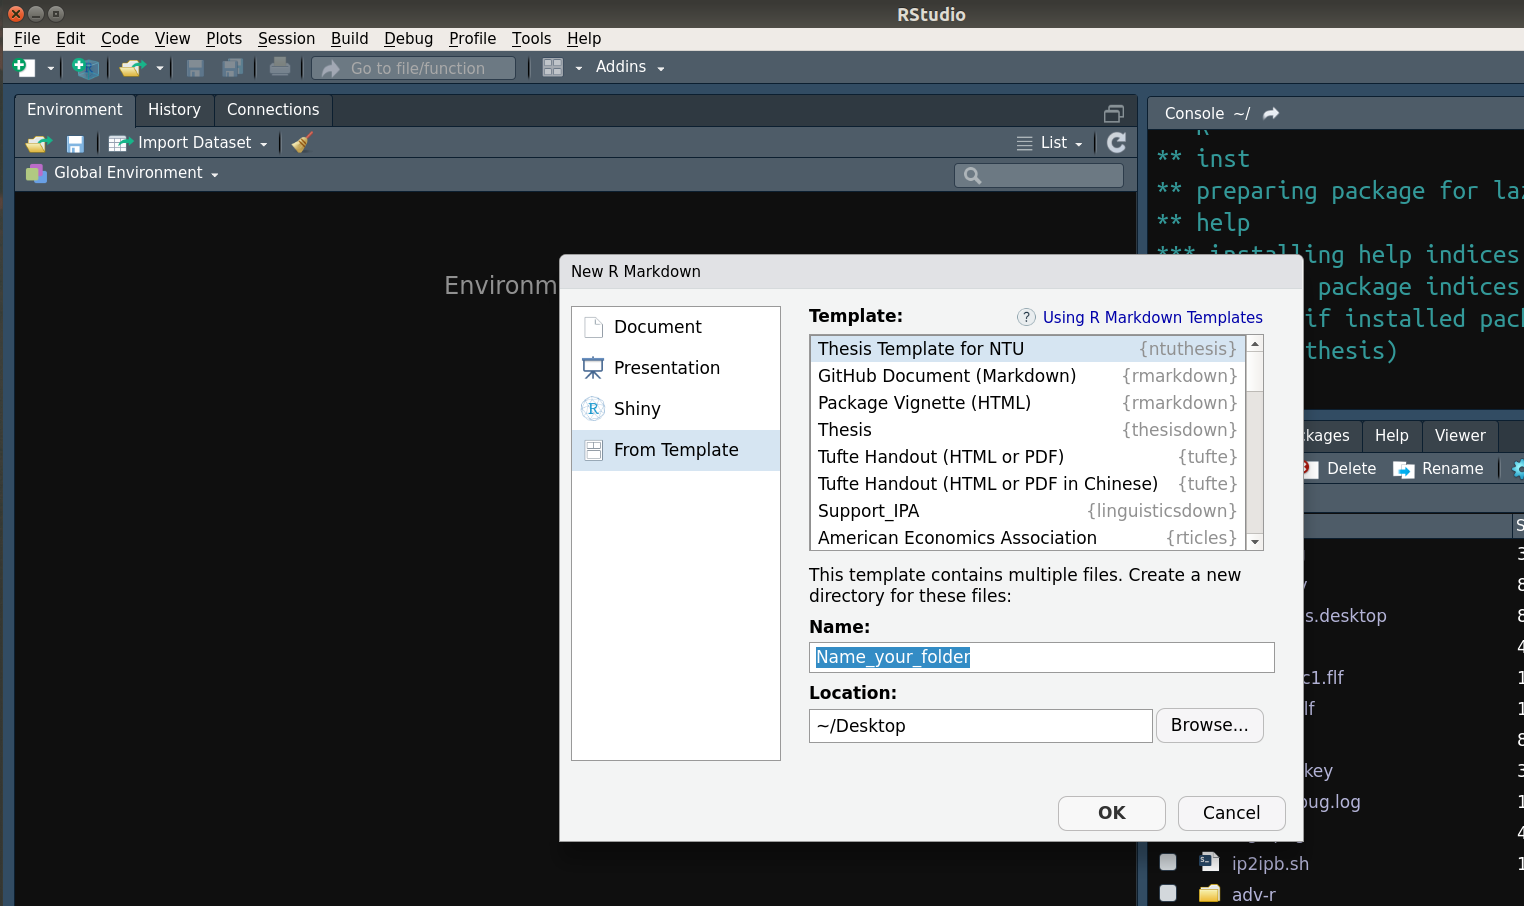
\includegraphics[width=0.9\linewidth]{figs/rmd-template} \end{center}

\begin{enumerate}
\def\labelenumi{\arabic{enumi}.}
\tightlist
\item
  選取左方\texttt{From\ Template}
\item
  找到\texttt{Thesis\ Template\ for\ NTU}
\item
  在下方\texttt{Name:}寫下欲創建之資料夾名稱
\end{enumerate}

或是直接在 console 執行:

\begin{Shaded}
\begin{Highlighting}[]
\NormalTok{rmarkdown}\OperatorTok{::}\KeywordTok{draft}\NormalTok{(}\StringTok{"project_name"}\NormalTok{,}
                 \DataTypeTok{template =} \StringTok{"ntu_bookdown"}\NormalTok{,}
                 \DataTypeTok{package =} \StringTok{"ntuthesis"}\NormalTok{)}
\end{Highlighting}
\end{Shaded}

接著需要將該資料夾變更為 bookdown 專案。這可以用 RStudio 左上方
\texttt{File} \textgreater{} \texttt{New\ Project} \textgreater{}
\texttt{Existing\ Directory} 達成,

或直接使用下方指令(working dir 需是專案資料夾):

\begin{Shaded}
\begin{Highlighting}[]
\NormalTok{ntuthesis}\OperatorTok{::}\KeywordTok{init_proj}\NormalTok{()  }\CommentTok{# init working dir as proj.}
\end{Highlighting}
\end{Shaded}

詳細的檔案結構,見第 \ref{dir-structure} 節。

\section{編輯封面}\label{edit-front-matter}

在\texttt{\_person-info.yml}輸入個人資料後,執行:

\begin{Shaded}
\begin{Highlighting}[]
\NormalTok{ntuthesis}\OperatorTok{::}\KeywordTok{comp_front}\NormalTok{()}
\end{Highlighting}
\end{Shaded}

即會在 \texttt{front-matter/}
生成封面所需的檔案。以使用者的角度而言,除了
\texttt{front-matter/certification.pdf} 以外,\texttt{front-matter/}
中的其它檔案不須理會。\texttt{certification.pdf}
是空白(未簽名)的「口試委員審定書」。

已簽名的「口試委員審定書」,將檔案命名為 \texttt{certification-scan.pdf}
並放在專案資料夾的最頂層。

\section{Compile 論文}\label{compile-thesis}

接著用 RStudio Environment Pane 裡的 button 輸出論文:

\begin{center}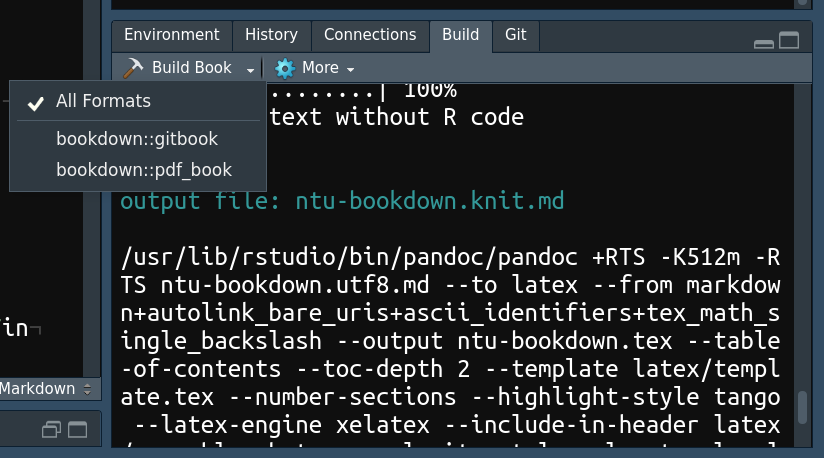
\includegraphics[width=0.9\linewidth]{figs/build-button} \end{center}

或是在 console 執行下方指令:

\begin{Shaded}
\begin{Highlighting}[]
\NormalTok{bookdown}\OperatorTok{::}\KeywordTok{render_book}\NormalTok{(}\StringTok{"index.Rmd"}\NormalTok{, }\StringTok{"bookdown::gitbook"}\NormalTok{)}
\NormalTok{bookdown}\OperatorTok{::}\KeywordTok{render_book}\NormalTok{(}\StringTok{"index.Rmd"}\NormalTok{, }\StringTok{"bookdown::bookdown::pdf_book"}\NormalTok{)}
\end{Highlighting}
\end{Shaded}

如此便會在 \texttt{\_book/} 中生成完整的論文(gitbook 和 PDF 格式)。

\chapter{論文撰寫}\label{write-thesis}

\section{檔案結構}\label{dir-structure}

執行以下指令後(詳見第 \ref{import-template} 節)

\begin{Shaded}
\begin{Highlighting}[]
\NormalTok{rmarkdown}\OperatorTok{::}\KeywordTok{draft}\NormalTok{(}\StringTok{"project_name"}\NormalTok{,}
                 \DataTypeTok{template =} \StringTok{"ntu_bookdown"}\NormalTok{,}
                 \DataTypeTok{package =} \StringTok{"ntuthesis"}\NormalTok{)}
\end{Highlighting}
\end{Shaded}

即會匯入論文模板,以下是論文模板的檔案結構(已簡化)。

\begin{Shaded}
\begin{Highlighting}[]
\NormalTok{├── project_name.Rmd     }\CommentTok{# Useless, please delete it}
\NormalTok{|}
\NormalTok{├── index.Rmd            }\CommentTok{# Book Layout (font, watermark, biblio, ...)}
\NormalTok{├── _acknowledge.Rmd     }\CommentTok{# acknowledgement}
\NormalTok{├── _abstract-en.Rmd     }\CommentTok{# abstract}
\NormalTok{├── _abstract-zh.Rmd     }\CommentTok{# Same as above, but in Chinese}
\NormalTok{|}
\NormalTok{├── 01-intro.Rmd         }\CommentTok{# Chapter 1 content}
\NormalTok{├── 02-literature.Rmd    }\CommentTok{# Chapter 2 content}
\NormalTok{├── 03-method.Rmd        }\CommentTok{# Chapter 3 content}
\NormalTok{├── 99-references.Rmd    }\CommentTok{# Don't need to edit}
\NormalTok{├── ref.bib              }\CommentTok{# References}
\NormalTok{├── cite-style.csl       }\CommentTok{# Citation style}
\NormalTok{|}
\NormalTok{├── _bookdown.yml        }\CommentTok{# label names in gitbook; Rmd files order}
\NormalTok{├── _output.yml          }\CommentTok{# preamble, pandoc args, cite-pkg}
\NormalTok{|}
\NormalTok{├── watermark.pdf        }\CommentTok{# 臺大浮水印 (PDF 右上角)}
\NormalTok{├── _person-info.yml      }\CommentTok{# Info to generate front matter}
\NormalTok{├── certification-scan.pdf  }\CommentTok{# 已簽名'口試委員審查書'}
\NormalTok{└── front_matter}
\NormalTok{    └── certification.pdf   }\CommentTok{# 空白'口試委員審查書'}
\end{Highlighting}
\end{Shaded}

\section{\texorpdfstring{\texttt{index.Rmd}}{index.Rmd}}\label{index.rmd}

\texttt{index.Rmd}

\section{撰寫語言}\label{write-lang}

若使用\textbf{英文}撰寫論文,需修改
\texttt{\_output.yml}、\texttt{\_bookdown.yml} 這兩個檔案的內容。

\subsection{\texorpdfstring{\texttt{\_output.yml}}{\_output.yml}}\label{output.yml}

將 \texttt{in\_header:\ latex/preamble-zh.tex} 改為
\texttt{in\_header:\ latex/preamble-en.tex}:

\begin{Shaded}
\begin{Highlighting}[]
\FunctionTok{bookdown:}\AttributeTok{:pdf_book:}
  \FunctionTok{includes:}
    \FunctionTok{in_header:}\AttributeTok{ latex/preamble-en.tex}
\end{Highlighting}
\end{Shaded}

\subsection{\texorpdfstring{\texttt{\_bookdown.yml}}{\_bookdown.yml}}\label{bookdown.yml}

\texttt{\_bookdown.yml} 中,可以對標籤的名稱進行定義。這裡的設定與 PDF
輸出無關,只與 gitbook 輸出格式有關。因此,若無需使用 gitbook
輸出,可忽略此段。

此外,\texttt{\_bookdown.yml} 亦可設定 Rmd
檔在輸出文件中的順序。若無設定,就會依序檔名排序\footnote{此模板即未進行設定,因此第一章的內容寫在
  \texttt{01-xxx.Rmd}
  就會自動排在第一。而若檔名以底線開頭(\texttt{\_})則會被忽略。更多內容詳見
  \href{https://bookdown.org/yihui/bookdown/usage.html}{bookdown}。}。

在以下設定中,可使 gitbook 輸出的章節(順序)與 PDF 不同。

\begin{Shaded}
\begin{Highlighting}[]
\FunctionTok{rmd_files:}
  \FunctionTok{html:}\AttributeTok{ }\KeywordTok{[}\StringTok{"index.Rmd"}\KeywordTok{,} \StringTok{"abstract.Rmd"}\KeywordTok{,} \StringTok{"intro.Rmd"}\KeywordTok{]}
  \FunctionTok{latex:}\AttributeTok{ }\KeywordTok{[}\StringTok{"abstract.Rmd"}\KeywordTok{,} \StringTok{"intro.Rmd"}\KeywordTok{]}
\end{Highlighting}
\end{Shaded}

\section{文獻引用}\label{bib-cite}

\begin{itemize}
\tightlist
\item
  csl
\item
  .bib
\item
  citr
\item
  limitation: bilingual
\end{itemize}

\chapter{Bookdown Cheatsheet}\label{bookdown-cheatsheet}

By default, bookdown merges all Rmd files by the order of filenames,
e.g., \texttt{01-intro.Rmd} will appear before
\texttt{02-literature.Rmd}. Filenames that start with an underscore
\texttt{\_} are skipped. \texttt{index.Rmd} will always be treated as
the first file.

\begin{itemize}
\tightlist
\item
  Benefits
\item
  Quick Start

  \begin{itemize}
  \tightlist
  \item
    General Usage

    \begin{itemize}
    \tightlist
    \item
      Front matter
    \item
      Content
    \end{itemize}
  \item
    Write Thesis in English (Write in Eng)
  \end{itemize}
\item
  Bookdown Demo

  \begin{enumerate}
  \def\labelenumi{\alph{enumi})}
  \tightlist
  \item
    Markdown quick guide

    \begin{itemize}
    \tightlist
    \item
      no closing or opening quotation marks
    \end{itemize}
  \item
    Citation
  \item
    Cross References
  \end{enumerate}

  \begin{itemize}
  \tightlist
  \item
    數學公式
  \item
    indexing
  \end{itemize}
\item
  Harnessing the Power of R Community

  \begin{enumerate}
  \def\labelenumi{\Alph{enumi})}
  \tightlist
  \item
    Facilitating Packages

    \begin{itemize}
    \tightlist
    \item
      citr
    \end{itemize}
  \item
    特定領域

    \begin{itemize}
    \tightlist
    \item
      linguisticsdown
    \end{itemize}
  \end{enumerate}
\item
  Resources

  \begin{itemize}
  \tightlist
  \item
    R Markdown Features
  \end{itemize}
\item
  Thanks and Help

  \begin{itemize}
  \tightlist
  \item
    GitHub issues
  \end{itemize}
\end{itemize}

\chapter{進階功能擴充}\label{add-on}

透過其它 R 套件,R Markdown
的撰寫過程能夠更順暢。以下介紹幾個例子,歡迎補充說明。

\section{語言學}\label{ling}

語言學相關文件寫作時,常需要插入 IPA
語音符號,但鍵盤通常難以直接打出這些符號。為此,我寫了一個 R
套件,讓使用者能直接在 RStudio 中透過輸入語音 features 的方式打出 IPA:

\begin{center}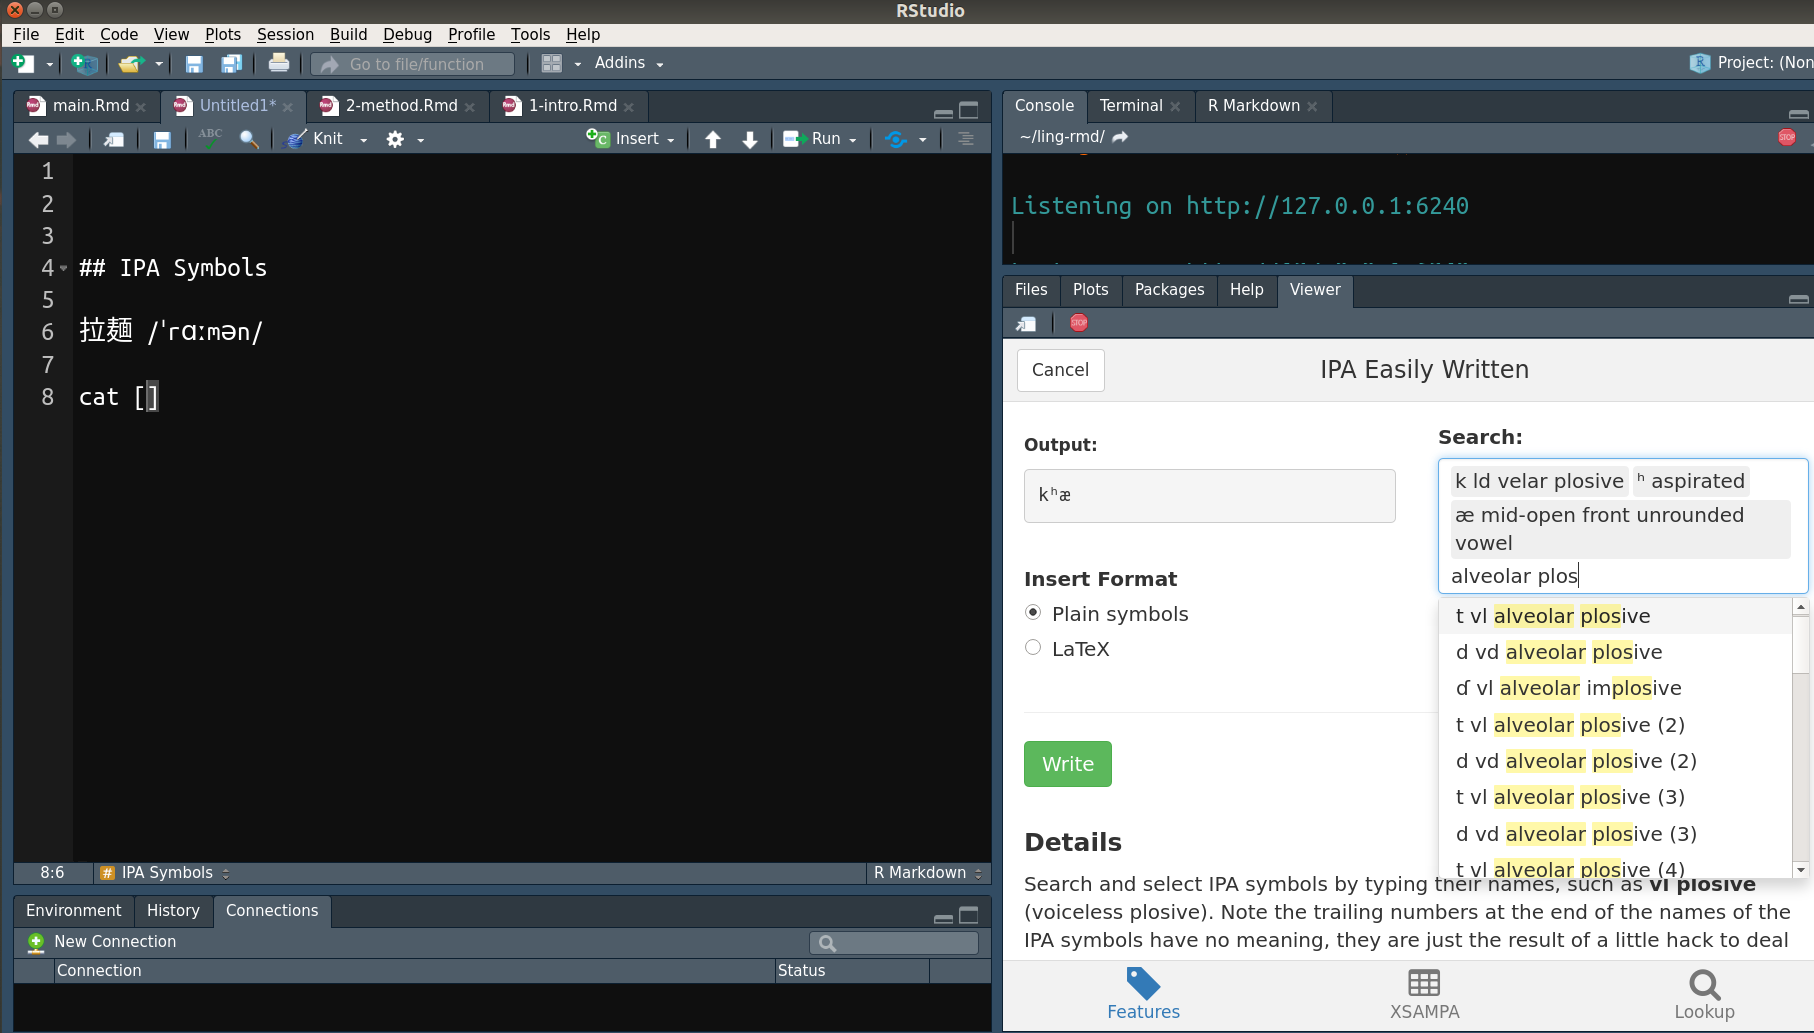
\includegraphics[width=0.9\linewidth]{figs/ipa} \end{center}

要使用這功能,需安裝 \texttt{linguisticsdown}:

\begin{Shaded}
\begin{Highlighting}[]
\KeywordTok{install.packages}\NormalTok{(}\StringTok{"linguisticsdown"}\NormalTok{)}
\end{Highlighting}
\end{Shaded}

並且在 \texttt{index.Rmd} 的 yaml 設定 IPA
符號專用的字型(需確認電腦上有安裝此字型):

\begin{Shaded}
\begin{Highlighting}[]
\FunctionTok{ipa-font:}\AttributeTok{ }\StringTok{'Doulos SIL'}
\end{Highlighting}
\end{Shaded}

關於更詳細的功能,見\href{https://liao961120.github.io/linguisticsdown/}{套件網頁}

\renewcommand{\href}{\oldhref}

\chapter*{參考資料}\label{references}
\addcontentsline{toc}{chapter}{參考資料}

\hypertarget{refs}{}
\hypertarget{ref-leung2008}{}
Leung, A. K.-y., Maddux, W. W., Galinsky, A. D., \& Chiu, C.-y. (2008).
Multicultural experience enhances creativity: The when and how.
\emph{American Psychologist}, \emph{63}(3), 169--181.
\url{https://doi.org/10.1037/0003-066X.63.3.169}

\hypertarget{ref-huangxuanfan1993}{}
黃宣範. (1993). \emph{語言、社會與族群意識: 臺灣語言社會學的研究}.
臺北市: 文鶴. Retrieved from
\url{http://tulips.ntu.edu.tw:1081/record=b1285025*cht}







\end{document}
